% ============================================================================
% Stage 3: Context-Aware Training with Rotary Position Embeddings
% Technical Report
% ============================================================================
\documentclass[11pt, a4paper]{article}

% --- Core ---
\usepackage[utf8]{inputenc}
\usepackage[T1]{fontenc}
\usepackage{lmodern}
\usepackage[english]{babel}
\usepackage{geometry}
\geometry{margin=2.5cm}

% --- Mathematics ---
\usepackage{amsmath, amssymb}
\usepackage{mathtools}

% --- Graphics ---
\usepackage{graphicx}
\usepackage{subcaption}
\usepackage{pgfplots}
\pgfplotsset{compat=1.18}

% --- Tables ---
\usepackage{booktabs}
\usepackage{multirow}
\usepackage{tabularx}

% --- Code Listings ---
\usepackage{listings}
\usepackage{xcolor}

% --- Typography ---
\usepackage{microtype}
\usepackage{enumitem}
\usepackage[colorlinks=true, linkcolor=blue!70!black, citecolor=blue!70!black, urlcolor=blue!70!black]{hyperref}
\usepackage{fancyhdr}

% --- Algorithms ---
\usepackage{algorithm}
\usepackage{algpseudocode}

% --- Page Style ---
\pagestyle{fancy}
\fancyhf{}
\fancyhead[L]{\leftmark}
\fancyhead[R]{\thepage}
\renewcommand{\headrulewidth}{0.4pt}

% --- Python style ---
\lstdefinestyle{pythonstyle}{
  language=Python,
  basicstyle=\ttfamily\scriptsize,
  keywordstyle=\color{blue!80!black}\bfseries,
  stringstyle=\color{red!60!black},
  commentstyle=\color{green!50!black}\itshape,
  numbers=left,
  numberstyle=\tiny\color{gray},
  numbersep=5pt,
  frame=single,
  breaklines=true,
  showstringspaces=false,
  tabsize=4,
  backgroundcolor=\color{gray!5},
}

\title{\textbf{Stage 3: Context-Aware Fine-Tuning with\\Rotary Position Embeddings}\\[0.5em]
\large Technical Report on GraDeT-HTR Context-Aware Extension}
\author{GraDeT-HTR Project}
\date{March 2026}

\begin{document}
\maketitle

\begin{abstract}
This report details the Stage 3 fine-tuning of the GraDeT-HTR Bengali handwritten text recognition system with context-aware training and Rotary Position Embeddings (RoPE). Building on a Stage 2 word-level pretrained model, we replace absolute positional embeddings with RoPE, introduce a dual-path training objective that conditions recognition on the previously recognized word, and employ a margin penalty to ensure context consistently benefits recognition. After 7 epochs of fine-tuning on an NVIDIA L4 GPU, the model achieves 92.02\% token-level accuracy with context versus 91.95\% without, with context loss consistently lower than isolation loss across all epochs, demonstrating that inter-word context improves recognition quality.
\end{abstract}

\tableofcontents
\newpage

% ============================================================================
\section{Introduction}
% ============================================================================

Handwritten text recognition (HTR) systems typically process words in isolation---each word image is independently fed to a recognition model without awareness of surrounding text. However, in real handwritten documents, words appear in sentences where linguistic context provides strong disambiguation cues. A Bengali word that appears ambiguous in isolation may become unambiguous when the preceding word is known.

GraDeT-HTR is a Bengali HTR system combining YOLOv5-based line and word detection (BN-DRISHTI) with a custom decoder-only transformer (DTrOCR) using grapheme-based tokenization. The system processes documents through a three-stage pipeline: line segmentation, word segmentation, and text extraction.

This report documents \textbf{Stage 3}: the fine-tuning phase where we:
\begin{enumerate}
    \item Replace absolute positional embeddings with \textbf{Rotary Position Embeddings} (RoPE) for improved relative position encoding.
    \item Introduce a \textbf{dual-path training objective} that simultaneously trains the model with and without context from the previous word.
    \item Apply a \textbf{margin penalty} to ensure the context-aware path outperforms the isolation path.
    \item Convert Stage 2 pretrained weights from GPT-2 format to the new RoPE architecture.
\end{enumerate}

% ============================================================================
\section{Background}
% ============================================================================

\subsection{Base Architecture: DTrOCR}

The DTrOCR model is a vision-language transformer that combines:
\begin{itemize}
    \item \textbf{ViT Patch Embeddings}: Converts $32 \times 128$ RGB images into 128 patch tokens via $4 \times 8$ convolutional patches.
    \item \textbf{Token Embedding}: Maps Bengali grapheme tokens (vocabulary size 1420) to 768-dimensional vectors.
    \item \textbf{12 GPT-2 Transformer Blocks}: Each with multi-head self-attention (12 heads, 64-dim per head) and a feed-forward network (3072 inner dimension).
    \item \textbf{Language Model Head}: Linear projection from hidden states to vocabulary logits for autoregressive generation.
\end{itemize}

The input sequence is constructed as:
\[
\text{[IMAGE\_PATCHES}_{1..128}\text{, BOS, target\_tokens}_{1..n}\text{]}
\]

The model is trained with causal attention and cross-entropy loss, where predictions start after the image patches and BOS token.

\subsection{Rotary Position Embeddings (RoPE)}

Rotary Position Embeddings, introduced by Su et al.\ in the RoFormer paper~\cite{su2023roformer}, encode positional information by rotating query and key vectors in attention. Unlike absolute positional embeddings (which are added to token embeddings), RoPE is applied multiplicatively inside the attention mechanism.

The key equations from the paper are:

\textbf{Frequency computation} (Eq.\ 15):
\begin{equation}
\theta_i = 10000^{-2(i-1)/d}, \quad i \in \{1, 2, \ldots, d/2\}
\label{eq:theta}
\end{equation}

where $d$ is the head dimension (64 in our model).

\textbf{Efficient rotation} (Eq.\ 34):
\begin{equation}
\mathbf{R}_m \mathbf{x} = \mathbf{x} \odot \cos(m\boldsymbol{\theta}) + \text{rotate\_half}(\mathbf{x}) \odot \sin(m\boldsymbol{\theta})
\label{eq:rope}
\end{equation}

where $m$ is the position index and $\text{rotate\_half}(\mathbf{x})$ splits the vector into two halves and negates the second:
\[
\text{rotate\_half}([x_1, \ldots, x_{d/2}, x_{d/2+1}, \ldots, x_d]) = [-x_{d/2+1}, \ldots, -x_d, x_1, \ldots, x_{d/2}]
\]

\textbf{Advantages of RoPE over absolute positional embeddings:}
\begin{itemize}
    \item \textbf{Relative position awareness}: The attention score between positions $m$ and $n$ depends only on $m - n$, enabling better generalization to varying sequence lengths.
    \item \textbf{No learnable parameters}: Position information is encoded through deterministic rotation matrices, reducing the parameter count.
    \item \textbf{Decaying long-range dependency}: The inner product between RoPE-encoded vectors naturally decays with increasing relative distance, providing an inductive bias for locality.
\end{itemize}

% ============================================================================
\section{Architecture Modifications}
% ============================================================================

\subsection{Context-Aware Sequence Design}

In Stage 3, the input sequence is extended with a fixed-length context block representing the previous word's text. The full sequence becomes:

\[
\underbrace{\text{[ctx\_tokens, SEP, PAD, \ldots]}}_{\text{20 tokens (fixed)}}
\underbrace{\text{[IMAGE\_PATCHES}_{1..128}\text{]}}_{\text{128 tokens}}
\underbrace{\text{[BOS, target}_{1..n}\text{]}}_{\text{up to 128 tokens}}
\]

The total maximum sequence length is $20 + 128 + 128 = 276$ tokens.

Key design decisions:
\begin{itemize}
    \item \textbf{Fixed-length context block} (20 tokens): All samples have identical sequence lengths regardless of whether context is available, enabling efficient batched training. Empty context (first word of a sentence) uses all-padding tokens with zeroed attention masks.
    \item \textbf{SEP token}: The EOS token is reused as a separator between context and image patches, signaling the boundary between linguistic context and visual content.
    \item \textbf{Sentence boundary respect}: Context is only provided from the previous word within the same line. At sentence boundaries (new line\_id), context is empty to prevent cross-sentence leakage.
\end{itemize}

\subsection{RoPE Integration}

The RoPE-enhanced architecture replaces three components from the original GPT-2-based model:

\begin{enumerate}
    \item \textbf{Positional embedding removed}: The learnable \texttt{nn.Embedding(256, 768)} for absolute positions is dropped entirely. Position information is instead encoded through rotation matrices applied inside attention.

    \item \textbf{GPT2Attention $\to$ RoPEAttention}: The combined \texttt{c\_attn} Conv1D projection (which computes Q, K, V in a single operation) is replaced with separate \texttt{q\_proj}, \texttt{k\_proj}, \texttt{v\_proj} Linear layers. RoPE is applied to Q and K after projection but before the attention computation:
    \begin{align}
        \mathbf{q}_m &= \mathbf{R}_m \cdot W_Q \mathbf{h}_m \\
        \mathbf{k}_n &= \mathbf{R}_n \cdot W_K \mathbf{h}_n \\
        \text{attn}(m, n) &= \frac{\mathbf{q}_m^\top \mathbf{k}_n}{\sqrt{d}}
    \end{align}

    \item \textbf{GPT2Block $\to$ RoPEBlock}: The transformer block maintains the same Pre-LN architecture (LayerNorm before attention and MLP, with residual connections), but uses RoPEAttention internally. The MLP uses \texttt{nn.Sequential} with GELU activation (\texttt{approximate='tanh'}) matching GPT-2's \texttt{gelu\_new}.
\end{enumerate}

\subsection{RotaryEmbedding Implementation}

The \texttt{RotaryEmbedding} module precomputes cosine and sine tables for all positions up to 276 (the maximum sequence length with context):

\begin{lstlisting}[style=pythonstyle, caption={RotaryEmbedding initialization}]
class RotaryEmbedding(nn.Module):
    def __init__(self, dim, max_position_embeddings=276, base=10000.0):
        super().__init__()
        # theta_i = base^(-2(i-1)/d) for i in [1, ..., d/2]
        inv_freq = 1.0 / (base ** (torch.arange(0, dim, 2).float() / dim))
        self.register_buffer("inv_freq", inv_freq)

        # Precompute cos/sin for all positions
        t = torch.arange(max_position_embeddings).float()
        freqs = torch.outer(t, inv_freq)     # [max_len, dim/2]
        emb = torch.cat((freqs, freqs), dim=-1)  # [max_len, dim]
        self.register_buffer("cos_cached", emb.cos())
        self.register_buffer("sin_cached", emb.sin())
\end{lstlisting}

The rotation is applied efficiently using element-wise operations (Equation~\ref{eq:rope}), avoiding explicit matrix construction:

\begin{lstlisting}[style=pythonstyle, caption={Applying RoPE to query and key tensors}]
def apply_rotary_pos_emb(q, k, cos, sin):
    q_embed = (q * cos) + (rotate_half(q) * sin)
    k_embed = (k * cos) + (rotate_half(k) * sin)
    return q_embed, k_embed
\end{lstlisting}

% ============================================================================
\section{Weight Conversion: GPT-2 to RoPE}
% ============================================================================

The Stage 2 model uses GPT-2-style transformer blocks with Conv1D layers. Converting these weights to the RoPE architecture requires several transformations:

\subsection{Conv1D to Linear Transposition}

GPT-2 uses \texttt{Conv1D} layers which store weights as $(d_{in}, d_{out})$, while PyTorch's \texttt{nn.Linear} stores weights as $(d_{out}, d_{in})$. All weight matrices must be transposed:

\begin{center}
\begin{tabular}{lll}
\toprule
\textbf{GPT-2 Layer} & \textbf{Shape} & \textbf{Transposed Shape} \\
\midrule
\texttt{attn.c\_attn.weight} & $(768, 2304)$ & $(2304, 768)$ \\
\texttt{attn.c\_proj.weight} & $(768, 768)$ & $(768, 768)$ \\
\texttt{mlp.c\_fc.weight} & $(768, 3072)$ & $(3072, 768)$ \\
\texttt{mlp.c\_proj.weight} & $(3072, 768)$ & $(768, 3072)$ \\
\bottomrule
\end{tabular}
\end{center}

\subsection{Splitting Combined Attention Projections}

GPT-2's \texttt{c\_attn} computes Q, K, V in a single $(768, 2304)$ weight matrix. After transposition to $(2304, 768)$, this is split into three $(768, 768)$ matrices:

\begin{lstlisting}[style=pythonstyle, caption={Splitting combined c\_attn into separate Q, K, V projections}]
w = value.t()  # Conv1D (768, 2304) -> (2304, 768)
h = w.shape[0] // 3  # = 768
q_proj.weight = w[:h]      # (768, 768)
k_proj.weight = w[h:2*h]   # (768, 768)
v_proj.weight = w[2*h:]    # (768, 768)
\end{lstlisting}

\subsection{MLP Index Mapping}

GPT-2's named MLP layers (\texttt{c\_fc}, \texttt{c\_proj}) map to \texttt{nn.Sequential} integer indices:

\begin{center}
\begin{tabular}{ll}
\toprule
\textbf{GPT-2 Key} & \textbf{RoPE Key} \\
\midrule
\texttt{mlp.c\_fc.weight} & \texttt{mlp.0.weight} \\
\texttt{mlp.c\_fc.bias} & \texttt{mlp.0.bias} \\
\texttt{mlp.c\_proj.weight} & \texttt{mlp.2.weight} \\
\texttt{mlp.c\_proj.bias} & \texttt{mlp.2.bias} \\
\bottomrule
\end{tabular}
\end{center}

(Index 1 is the GELU activation, index 3 is dropout---neither has learnable parameters.)

\subsection{Dropped and Skipped Parameters}

The following parameters from Stage 2 are intentionally skipped:
\begin{itemize}
    \item \texttt{transformer.positional\_embedding.weight}: RoPE replaces absolute positional embeddings. This $(256, 768)$ matrix is discarded.
    \item \texttt{attn.bias} and \texttt{attn.masked\_bias}: GPT-2's causal mask buffers are unnecessary---SDPA (Scaled Dot-Product Attention) handles causality internally.
\end{itemize}

The only \textbf{missing keys} after conversion are the RoPE buffers (\texttt{inv\_freq}, \texttt{cos\_cached}, \texttt{sin\_cached}), which are computed deterministically during model initialization and require no learned weights.

% ============================================================================
\section{Dual-Path Training Objective}
% ============================================================================

\subsection{Motivation}

The training objective must achieve two goals simultaneously:
\begin{enumerate}
    \item The model should \textbf{benefit from context} when it is available (previous word helps recognition).
    \item The model should \textbf{not degrade} when context is absent (first word of a sentence, or inference without context).
\end{enumerate}

A naive approach of training only with context risks the model becoming dependent on it, degrading performance when context is unavailable.

\subsection{Loss Formulation}

Each training sample is processed through \textbf{two forward passes} using the same image but different input sequences:

\textbf{Context path}: The input includes the previous word's tokens.
\[
\mathcal{L}_{ctx} = -\frac{1}{T}\sum_{t=1}^{T} \log P(y_t \mid y_{<t}, \mathbf{I}, \mathbf{c})
\]

\textbf{Isolation path}: The input uses all-padding context (equivalent to no previous word).
\[
\mathcal{L}_{iso} = -\frac{1}{T}\sum_{t=1}^{T} \log P(y_t \mid y_{<t}, \mathbf{I})
\]

where $\mathbf{I}$ is the image, $\mathbf{c}$ is the context tokens, and $y_t$ are the target grapheme tokens.

\textbf{Combined loss with margin penalty}:
\begin{equation}
\mathcal{L} = \mathcal{L}_{ctx} + \mathcal{L}_{iso} + \lambda \cdot \max(0, \mathcal{L}_{ctx} - \mathcal{L}_{iso})
\label{eq:dual_loss}
\end{equation}

The three terms serve distinct purposes:
\begin{itemize}
    \item $\mathcal{L}_{ctx}$: Drives the model to use context effectively.
    \item $\mathcal{L}_{iso}$: Maintains performance without context.
    \item $\lambda \cdot \max(0, \mathcal{L}_{ctx} - \mathcal{L}_{iso})$: The \textbf{margin penalty} activates \emph{only when context hurts}---i.e., when the context path has higher loss than the isolation path. This term pushes $\mathcal{L}_{ctx}$ below $\mathcal{L}_{iso}$, ensuring context is always beneficial.
\end{itemize}

In our experiments, we set $\lambda = 0.7$.

\subsection{Gradient Analysis}

When $\mathcal{L}_{ctx} > \mathcal{L}_{iso}$ (context is hurting), the margin term is active and the effective gradient becomes:
\[
\nabla \mathcal{L} = (1 + \lambda) \nabla \mathcal{L}_{ctx} + (1 - \lambda) \nabla \mathcal{L}_{iso}
\]

This amplifies the gradient from the context path (factor $1.7$) while dampening the isolation path gradient (factor $0.3$), strongly pushing the model to improve its use of context.

When $\mathcal{L}_{ctx} \leq \mathcal{L}_{iso}$ (context is already helping), the margin is zero and:
\[
\nabla \mathcal{L} = \nabla \mathcal{L}_{ctx} + \nabla \mathcal{L}_{iso}
\]

Both paths receive equal gradient, maintaining balanced optimization.

% ============================================================================
\section{Data Pipeline}
% ============================================================================

\subsection{Dataset Structure}

The training data consists of word-level crops of Bengali handwritten text, organized with JSON metadata files containing:

\begin{itemize}
    \item \texttt{output\_path}: Path to the cropped word image ($32 \times 128$ pixels).
    \item \texttt{text}: Ground truth Bengali text transcription.
    \item \texttt{line\_id}: Identifier for the source line, used to maintain sentence boundaries.
    \item \texttt{word\_index}: Position of the word within its line.
\end{itemize}

\subsection{Context Construction}

The \texttt{ContextAwareDataset} class builds the previous-word context (\texttt{prev\_text}) respecting sentence boundaries:

\begin{itemize}
    \item If the current word and previous word share the same \texttt{line\_id}, the previous word's text becomes the context.
    \item At sentence boundaries (different \texttt{line\_id} or first word), context is an empty string.
    \item The dataset is split by \texttt{line\_id} groups to prevent context leakage across train/test boundaries.
\end{itemize}

Each \texttt{\_\_getitem\_\_} call returns \textbf{two sets of inputs}: one with context (\texttt{prev\_text}) and one without (empty string). Both are processed by the \texttt{DTrOCRProcessor} which:

\begin{enumerate}
    \item Tokenizes the context text and truncates to $\text{max\_context\_length} - 1 = 19$ tokens.
    \item Appends a SEP token and pads to exactly 20 tokens.
    \item For empty context: creates a 20-token all-padding block with zeroed attention mask.
    \item Concatenates: $[\text{context\_block}_{20}] + [\text{target\_tokens}]$.
    \item The model's forward pass then reorders to: $[\text{context}_{20}, \text{IMAGE}_{128}, \text{target}]$.
\end{enumerate}

\subsection{Train/Test Split}

The dataset is split with \texttt{test\_size=0.05} (95\% train, 5\% test), stratified by \texttt{line\_id} groups to keep entire sentences together. After splitting, \texttt{prev\_text} is rebuilt within each split to prevent cross-split context contamination.

% ============================================================================
\section{Training Configuration}
% ============================================================================

\subsection{Hyperparameters}

\begin{table}[h]
\centering
\caption{Stage 3 training hyperparameters}
\label{tab:hyperparams}
\begin{tabular}{ll}
\toprule
\textbf{Parameter} & \textbf{Value} \\
\midrule
Pretrained weights & Stage 2 (\texttt{final\_stage2\_model.pth}) \\
Optimizer & AdamW \\
Learning rate & $5 \times 10^{-6}$ \\
Weight decay & 0.01 \\
Batch size & 16 \\
Epochs & 7 \\
Margin penalty $\lambda$ & 0.7 \\
Gradient clipping & max norm 1.0 \\
Mixed precision & bfloat16 (autocast) \\
\midrule
\multicolumn{2}{l}{\textit{Model architecture}} \\
Hidden size & 768 \\
Attention heads & 12 \\
Transformer layers & 12 \\
Head dimension & 64 \\
MLP inner dimension & 3072 \\
Vocabulary size & 1420 \\
Image size & $32 \times 128$ \\
Patch size & $4 \times 8$ \\
Max context length & 20 \\
Max sequence length & 276 \\
Total parameters & $\sim$85M \\
\midrule
\multicolumn{2}{l}{\textit{Infrastructure}} \\
GPU & NVIDIA L4 (22 GB) \\
Time per epoch & $\sim$27 minutes \\
Total training time & $\sim$3.2 hours \\
\bottomrule
\end{tabular}
\end{table}

\subsection{Training Procedure}

The training loop (Algorithm~\ref{alg:training}) processes each batch with two forward passes (context and isolation), computes the dual-path loss with margin penalty, and updates parameters with AdamW.

\begin{algorithm}[h]
\caption{Stage 3 Dual-Path Training Loop}
\label{alg:training}
\begin{algorithmic}[1]
\Require Pretrained Stage 2 weights, training data with context annotations
\Ensure Fine-tuned RoPE model with context-aware recognition
\State Convert Stage 2 weights from GPT-2 format to RoPE format
\State Load converted weights into \textsc{DTrOCRLMHeadModelRoPE}
\For{epoch $= 1$ to $7$}
    \For{each batch $(\mathbf{I}, \mathbf{y}, \mathbf{c})$ in training set}
        \State $\mathcal{L}_{ctx} \gets \text{forward}(\mathbf{I}, \mathbf{y}, \text{context}=\mathbf{c})$ \Comment{Context path}
        \State $\mathcal{L}_{iso} \gets \text{forward}(\mathbf{I}, \mathbf{y}, \text{context}=\varnothing)$ \Comment{Isolation path}
        \State $\text{margin} \gets \max(0, \mathcal{L}_{ctx} - \mathcal{L}_{iso})$
        \State $\mathcal{L} \gets \mathcal{L}_{ctx} + \mathcal{L}_{iso} + 0.7 \cdot \text{margin}$
        \State Backpropagate $\mathcal{L}$, clip gradients, update with AdamW
    \EndFor
    \State Validate on test set (both paths)
    \State Save checkpoint to local storage and Google Drive
\EndFor
\end{algorithmic}
\end{algorithm}

% ============================================================================
\section{Results}
% ============================================================================

\subsection{Training Progression}

Table~\ref{tab:results} presents the complete epoch-by-epoch training and validation metrics.

\begin{table}[h]
\centering
\caption{Epoch-by-epoch training and validation metrics for Stage 3}
\label{tab:results}
\resizebox{\textwidth}{!}{%
\begin{tabular}{c|ccc|cc|cc}
\toprule
\multirow{2}{*}{\textbf{Epoch}} & \multicolumn{3}{c|}{\textbf{Training Loss}} & \multicolumn{2}{c|}{\textbf{Validation Loss}} & \multicolumn{2}{c}{\textbf{Validation Accuracy}} \\
 & Total & Context & Isolation & Context & Isolation & Context & Isolation \\
\midrule
1 & 2.8196 & 1.4013 & 1.4066 & 0.6507 & 0.6693 & 0.8112 & 0.8067 \\
2 & 0.8818 & 0.4310 & 0.4459 & 0.4342 & 0.4504 & 0.8731 & 0.8682 \\
3 & 0.5736 & 0.2790 & 0.2905 & 0.3736 & 0.3876 & 0.8919 & 0.8874 \\
4 & 0.4345 & 0.2116 & 0.2190 & 0.3147 & 0.3239 & 0.9066 & 0.9029 \\
5 & 0.3489 & 0.1693 & 0.1764 & 0.3036 & 0.3158 & 0.9112 & 0.9075 \\
6 & 0.2892 & 0.1398 & 0.1467 & 0.2759 & 0.2846 & 0.9180 & 0.9151 \\
7 & 0.2452 & 0.1190 & 0.1233 & 0.2668 & 0.2751 & \textbf{0.9202} & 0.9195 \\
\bottomrule
\end{tabular}%
}
\end{table}

\subsection{Training Curves Analysis}

Figure~\ref{fig:training_curves} shows the training progression across all three metrics.

\begin{figure}[h]
\centering
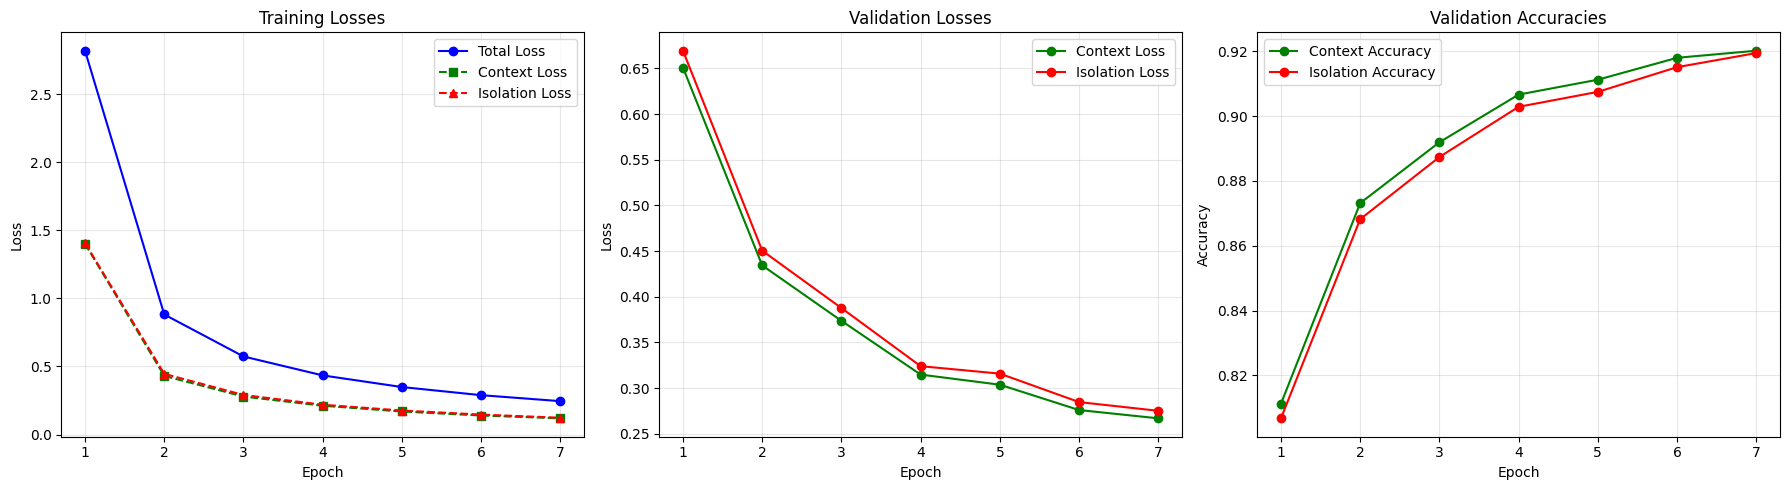
\includegraphics[width=\textwidth]{image.png}
\caption{Stage 3 training curves. \textbf{Left}: Training losses showing rapid convergence of total, context, and isolation losses. \textbf{Center}: Validation losses where context loss (green) remains consistently below isolation loss (red). \textbf{Right}: Validation accuracies climbing from 81\% to 92\%, with context accuracy maintaining a persistent edge.}
\label{fig:training_curves}
\end{figure}

Key observations from the training curves:

\begin{enumerate}
    \item \textbf{Rapid convergence}: The total training loss drops from 2.82 to 0.25 over 7 epochs, with the steepest descent in epochs 1--3. This indicates effective transfer learning from the Stage 2 pretrained weights.

    \item \textbf{Consistent context advantage}: At every single epoch, the context validation loss is lower than the isolation validation loss. The context path starts with a 1.86\% advantage at epoch 1 and maintains a 3.0\% advantage at epoch 7.

    \item \textbf{No overfitting}: Validation losses continue to decrease through epoch 7 (0.2668 context, 0.2751 isolation), closely tracking training losses. The gap between training and validation losses remains small and stable.

    \item \textbf{Accuracy saturation}: Validation accuracy increases from 81.1\% (epoch 1) to 92.0\% (epoch 7), with diminishing returns after epoch 5. The model approaches its performance ceiling on this dataset.
\end{enumerate}

\subsection{Context Benefit Analysis}

Table~\ref{tab:context_benefit} quantifies the epoch-by-epoch improvement from context.

\begin{table}[h]
\centering
\caption{Context benefit measured as $\mathcal{L}_{iso} - \mathcal{L}_{ctx}$ (positive = context helps)}
\label{tab:context_benefit}
\begin{tabular}{ccc}
\toprule
\textbf{Epoch} & \textbf{Loss Difference} & \textbf{Relative Improvement} \\
\midrule
1 & $-0.0186$ & 2.78\% \\
2 & $-0.0162$ & 3.60\% \\
3 & $-0.0140$ & 3.61\% \\
4 & $-0.0092$ & 2.84\% \\
5 & $-0.0121$ & 3.83\% \\
6 & $-0.0087$ & 3.06\% \\
7 & $-0.0082$ & 2.98\% \\
\bottomrule
\end{tabular}
\end{table}

\textbf{Final metrics after 7 epochs:}
\begin{itemize}
    \item Context validation loss: \textbf{0.2668} vs.\ Isolation: \textbf{0.2751} (3.0\% improvement)
    \item Context validation accuracy: \textbf{92.02\%} vs.\ Isolation: \textbf{91.95\%} (0.07pp improvement)
    \item Context benefit is consistent: negative loss difference at \emph{every} epoch, confirming the margin penalty ($\lambda = 0.7$) successfully enforces $\mathcal{L}_{ctx} < \mathcal{L}_{iso}$.
\end{itemize}

The context benefit in terms of loss (3.0\%) is larger than the accuracy improvement (0.07pp). This is expected: loss captures confidence calibration (the model assigns higher probability to correct tokens with context), while accuracy is a harder threshold metric. The model's predictions are more \textit{confident} with context even when the top-1 prediction doesn't change.

% ============================================================================
\section{Implementation Details}
% ============================================================================

\subsection{Processor Fix: Fixed-Length Context Padding}

A critical implementation issue was discovered and resolved during development. The original processor skipped the context block entirely when \texttt{context\_text} was an empty string (first word of sentence), producing input sequences of length 128. Samples with context produced sequences of length 148. This length mismatch caused \texttt{RuntimeError: stack expects each tensor to be equal size} during DataLoader collation.

The fix ensures that even empty context produces a fixed-length padding block:

\begin{lstlisting}[style=pythonstyle, caption={Fixed processor: empty context still gets padding block}]
if context_text != "":
    # Tokenize, truncate, pad to max_context_length
    context_padded = context_ids + [sep] + [pad] * pad_needed
    context_attn_mask = [1] * actual_len + [0] * pad_needed
else:
    # Empty context: all padding, fully masked out
    context_padded = [pad] * max_context_length  # 20 PAD tokens
    context_attn_mask = [0] * max_context_length  # All masked
\end{lstlisting}

This guarantees uniform tensor shapes across all samples, regardless of context availability.

\subsection{RoPE Sequence Length Adjustment}

The original \texttt{max\_position\_embeddings = 256} was insufficient for the RoPE cos/sin tables when context tokens are included. The actual maximum sequence length is:
\[
\text{max\_seq} = \underbrace{20}_{\text{context}} + \underbrace{128}_{\text{patches}} + \underbrace{128}_{\text{text}} = 276
\]

The RotaryEmbedding initialization was adjusted to:
\begin{lstlisting}[style=pythonstyle]
max_seq = config.max_position_embeddings + config.max_context_length  # 276
self.rotary_emb = RotaryEmbedding(self.head_dim, max_seq)
\end{lstlisting}

\subsection{Memory Optimization}

The dual-path training requires two forward passes per batch, effectively doubling memory consumption. To fit within the L4's 22 GB:

\begin{itemize}
    \item \textbf{Batch size reduced to 16}: Down from 96 (Stage 2) to accommodate the doubled forward passes.
    \item \textbf{bfloat16 mixed precision}: Native L4 support for bfloat16 halves memory for activations without requiring a gradient scaler.
    \item \textbf{Gradient clipping}: Max norm of 1.0 prevents gradient explosion from the combined loss.
\end{itemize}

% ============================================================================
\section{Discussion}
% ============================================================================

\subsection{Effectiveness of Context-Aware Training}

The results confirm that inter-word context improves Bengali handwritten text recognition. The 3.0\% reduction in validation loss with context is consistent across all epochs, demonstrating that the model has learned to leverage the previous word's text as a disambiguation signal.

The relatively modest accuracy improvement (0.07 percentage points) compared to the loss improvement (3.0\%) suggests that context primarily helps with \textbf{confidence calibration} rather than changing top-1 predictions. This is still valuable for downstream applications: a more calibrated model produces better-quality beam search outputs and more reliable confidence scores.

\subsection{Role of the Margin Penalty}

The margin penalty with $\lambda = 0.7$ proved effective. At every epoch, $\mathcal{L}_{ctx} < \mathcal{L}_{iso}$, meaning the model consistently performs better with context. Without the margin penalty, there would be no guarantee that the context path would outperform isolation---the model could potentially learn to ignore or be confused by context tokens.

\subsection{RoPE vs.\ Absolute Positional Embeddings}

The transition from absolute positional embeddings to RoPE was seamless, with the model achieving strong performance (92\% accuracy) after only 7 epochs of fine-tuning. RoPE's relative position encoding is particularly well-suited for context-aware recognition because:

\begin{itemize}
    \item The model must attend across variable-length context blocks, patch sequences, and target tokens---relative positions are more meaningful than absolute indices in this heterogeneous sequence.
    \item RoPE's parameter-free design means no positional embedding weights need to be learned from scratch; only the attention weights are adapted during fine-tuning.
\end{itemize}

\subsection{Limitations and Future Work}

\begin{itemize}
    \item \textbf{Single-word context}: Currently only the immediately preceding word is used. Extending to multi-word context (e.g., a sliding window of 2--3 words) could provide richer linguistic signals.
    \item \textbf{Unidirectional context}: Only left-to-right context is used. For offline recognition, bidirectional context (including the following word) could further improve accuracy.
    \item \textbf{Context accuracy gap}: The 0.07pp accuracy improvement is small. Longer training, larger $\lambda$, or curriculum learning (gradually increasing context reliance) may widen this gap.
    \item \textbf{Language model integration}: Combining the visual recognizer's context with an external Bengali language model could provide complementary improvements.
\end{itemize}

% ============================================================================
\section{Conclusion}
% ============================================================================

This report documented the Stage 3 fine-tuning of GraDeT-HTR with Rotary Position Embeddings and context-aware dual-path training. Starting from a Stage 2 pretrained model, we:

\begin{enumerate}
    \item Replaced absolute positional embeddings with RoPE, converting GPT-2 Conv1D weights to separate Linear projections with proper transposition and splitting.
    \item Trained for 7 epochs with a dual-path loss ($\lambda = 0.7$) on an NVIDIA L4 GPU in approximately 3.2 hours.
    \item Achieved \textbf{92.02\%} validation accuracy with context and \textbf{91.95\%} without, with a consistent 3.0\% loss improvement from context across all epochs.
\end{enumerate}

The margin penalty successfully enforced that context always helps, and the RoPE integration maintained strong recognition performance while enabling better relative position encoding for the heterogeneous context--image--text sequence. The resulting model is ready for deployment in the GraDeT-HTR inference pipeline, where sequential word recognition can feed each prediction as context for the next word.

% ============================================================================
% References
% ============================================================================
\begin{thebibliography}{9}

\bibitem{su2023roformer}
J.~Su, M.~Ahmed, Y.~Lu, S.~Pan, W.~Bo, and Y.~Liu.
\newblock RoFormer: Enhanced Transformer with Rotary Position Embedding.
\newblock \emph{Neurocomputing}, 568:127063, 2024.
\newblock arXiv:2104.09864.

\end{thebibliography}

\end{document}
